%\Preamble
\documentclass[a4paper,12pt,]{article}
\usepackage{amsmath}
\usepackage{graphicx}
\graphicspath{ {./images/} }

%Actual document content
\begin{document}
	
	\title{First Document}
	\author{Vasudev Kini}
	\date{\today}
	\maketitle
	
	\textsc{Quote}  \\ % \\ Stands for new line
	Some of the \textbf{greatest}
	discoveries in \underline{science} 
	were made by \textbf{\textit{accident}}.
	
	\begin{figure}
		%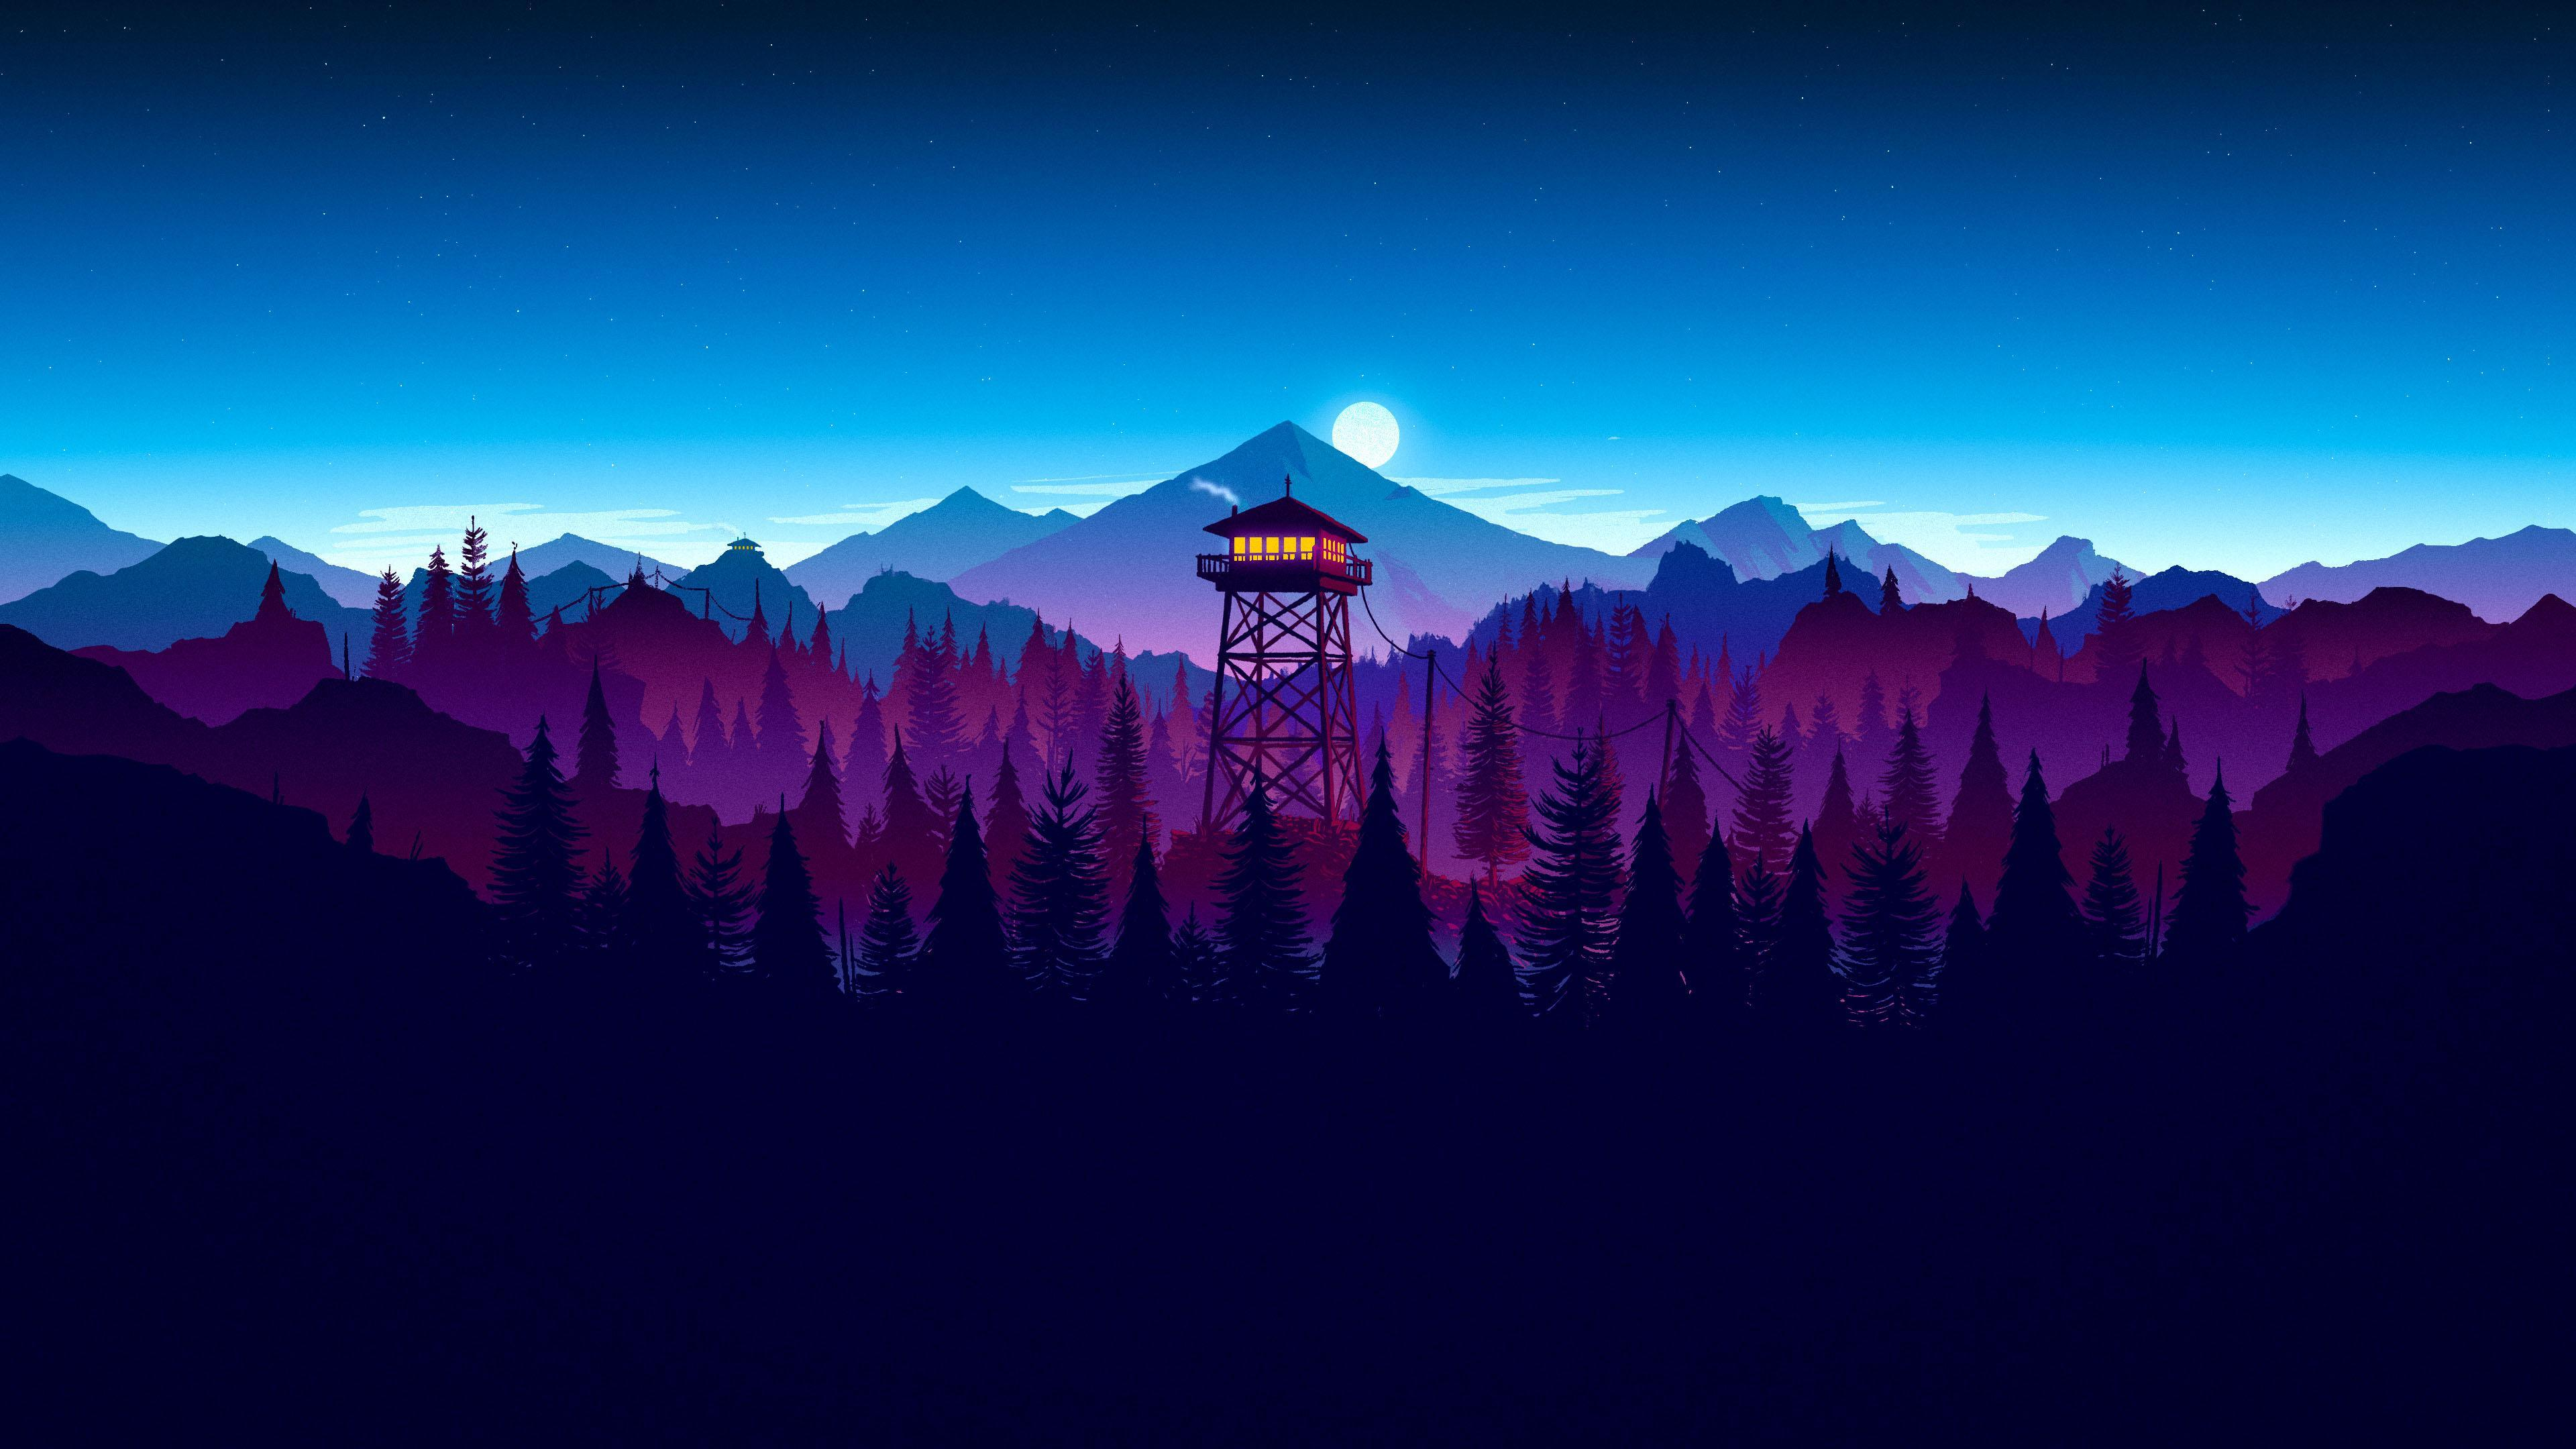
\includegraphics[width=150mm,scale=0.5]{wallaper.jpg}
		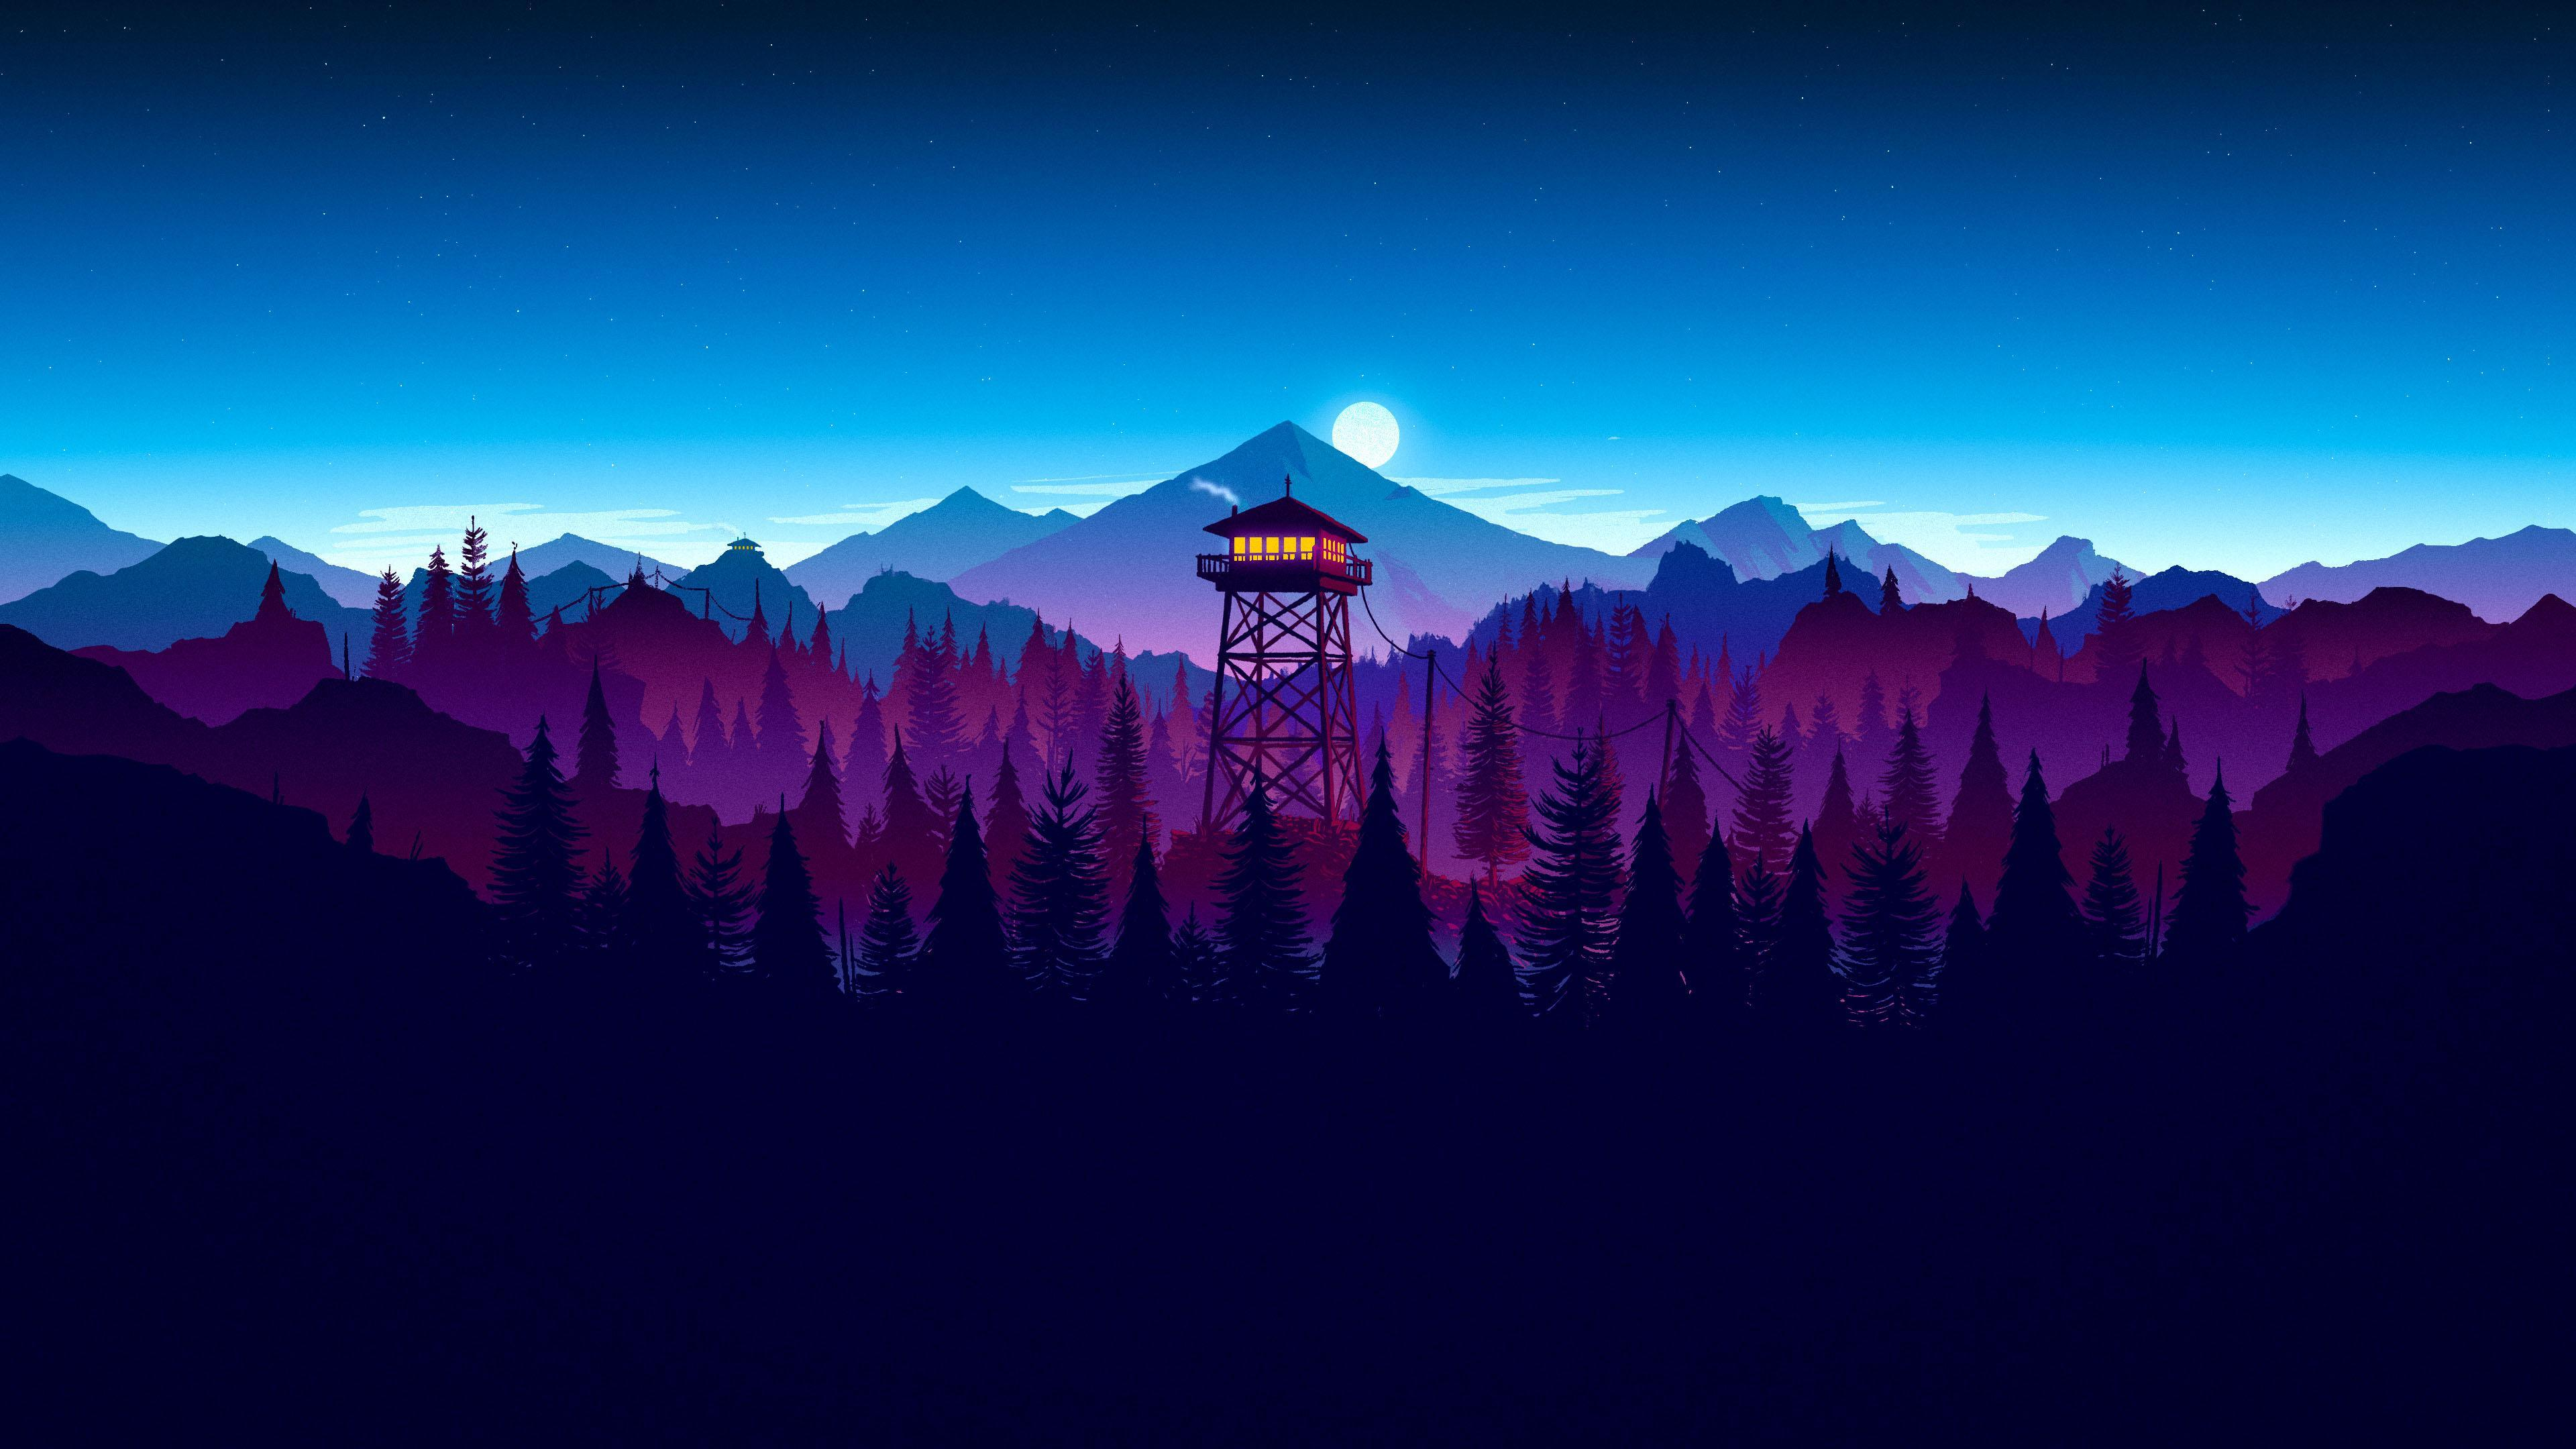
\includegraphics[width=0.25\textwidth]{wallaper.jpg}
	 	\centering
		\caption{a nice plot}
		\label{fig:mesh1}
	\end{figure}

	As you can see in the figure \ref{fig:mesh1}, the 
	function grows near 0. Also, in the page \pageref{fig:mesh1} 
	is the same example.
	
	Heloooo

\end{document}